% Options for packages loaded elsewhere
\PassOptionsToPackage{unicode}{hyperref}
\PassOptionsToPackage{hyphens}{url}
%
\documentclass[
]{book}
\usepackage{lmodern}
\usepackage{amssymb,amsmath}
\usepackage{ifxetex,ifluatex}
\ifnum 0\ifxetex 1\fi\ifluatex 1\fi=0 % if pdftex
  \usepackage[T1]{fontenc}
  \usepackage[utf8]{inputenc}
  \usepackage{textcomp} % provide euro and other symbols
\else % if luatex or xetex
  \usepackage{unicode-math}
  \defaultfontfeatures{Scale=MatchLowercase}
  \defaultfontfeatures[\rmfamily]{Ligatures=TeX,Scale=1}
\fi
% Use upquote if available, for straight quotes in verbatim environments
\IfFileExists{upquote.sty}{\usepackage{upquote}}{}
\IfFileExists{microtype.sty}{% use microtype if available
  \usepackage[]{microtype}
  \UseMicrotypeSet[protrusion]{basicmath} % disable protrusion for tt fonts
}{}
\makeatletter
\@ifundefined{KOMAClassName}{% if non-KOMA class
  \IfFileExists{parskip.sty}{%
    \usepackage{parskip}
  }{% else
    \setlength{\parindent}{0pt}
    \setlength{\parskip}{6pt plus 2pt minus 1pt}}
}{% if KOMA class
  \KOMAoptions{parskip=half}}
\makeatother
\usepackage{xcolor}
\IfFileExists{xurl.sty}{\usepackage{xurl}}{} % add URL line breaks if available
\IfFileExists{bookmark.sty}{\usepackage{bookmark}}{\usepackage{hyperref}}
\hypersetup{
  pdftitle={Ocean Health Index for northern Norway},
  pdfauthor={Marina Espinasse},
  hidelinks,
  pdfcreator={LaTeX via pandoc}}
\urlstyle{same} % disable monospaced font for URLs
\usepackage{longtable,booktabs}
% Correct order of tables after \paragraph or \subparagraph
\usepackage{etoolbox}
\makeatletter
\patchcmd\longtable{\par}{\if@noskipsec\mbox{}\fi\par}{}{}
\makeatother
% Allow footnotes in longtable head/foot
\IfFileExists{footnotehyper.sty}{\usepackage{footnotehyper}}{\usepackage{footnote}}
\makesavenoteenv{longtable}
\usepackage{graphicx}
\makeatletter
\def\maxwidth{\ifdim\Gin@nat@width>\linewidth\linewidth\else\Gin@nat@width\fi}
\def\maxheight{\ifdim\Gin@nat@height>\textheight\textheight\else\Gin@nat@height\fi}
\makeatother
% Scale images if necessary, so that they will not overflow the page
% margins by default, and it is still possible to overwrite the defaults
% using explicit options in \includegraphics[width, height, ...]{}
\setkeys{Gin}{width=\maxwidth,height=\maxheight,keepaspectratio}
% Set default figure placement to htbp
\makeatletter
\def\fps@figure{htbp}
\makeatother
\setlength{\emergencystretch}{3em} % prevent overfull lines
\providecommand{\tightlist}{%
  \setlength{\itemsep}{0pt}\setlength{\parskip}{0pt}}
\setcounter{secnumdepth}{5}
\usepackage{booktabs}
\usepackage{amsthm}
\makeatletter
\def\thm@space@setup{%
  \thm@preskip=8pt plus 2pt minus 4pt
  \thm@postskip=\thm@preskip
}
\makeatother
\usepackage[]{natbib}
\bibliographystyle{apalike}

\title{Ocean Health Index for northern Norway}
\author{Marina Espinasse}
\date{2020-02-28}

\begin{document}
\maketitle

{
\setcounter{tocdepth}{1}
\tableofcontents
}
\hypertarget{about-the-project}{%
\chapter{About the project}\label{about-the-project}}

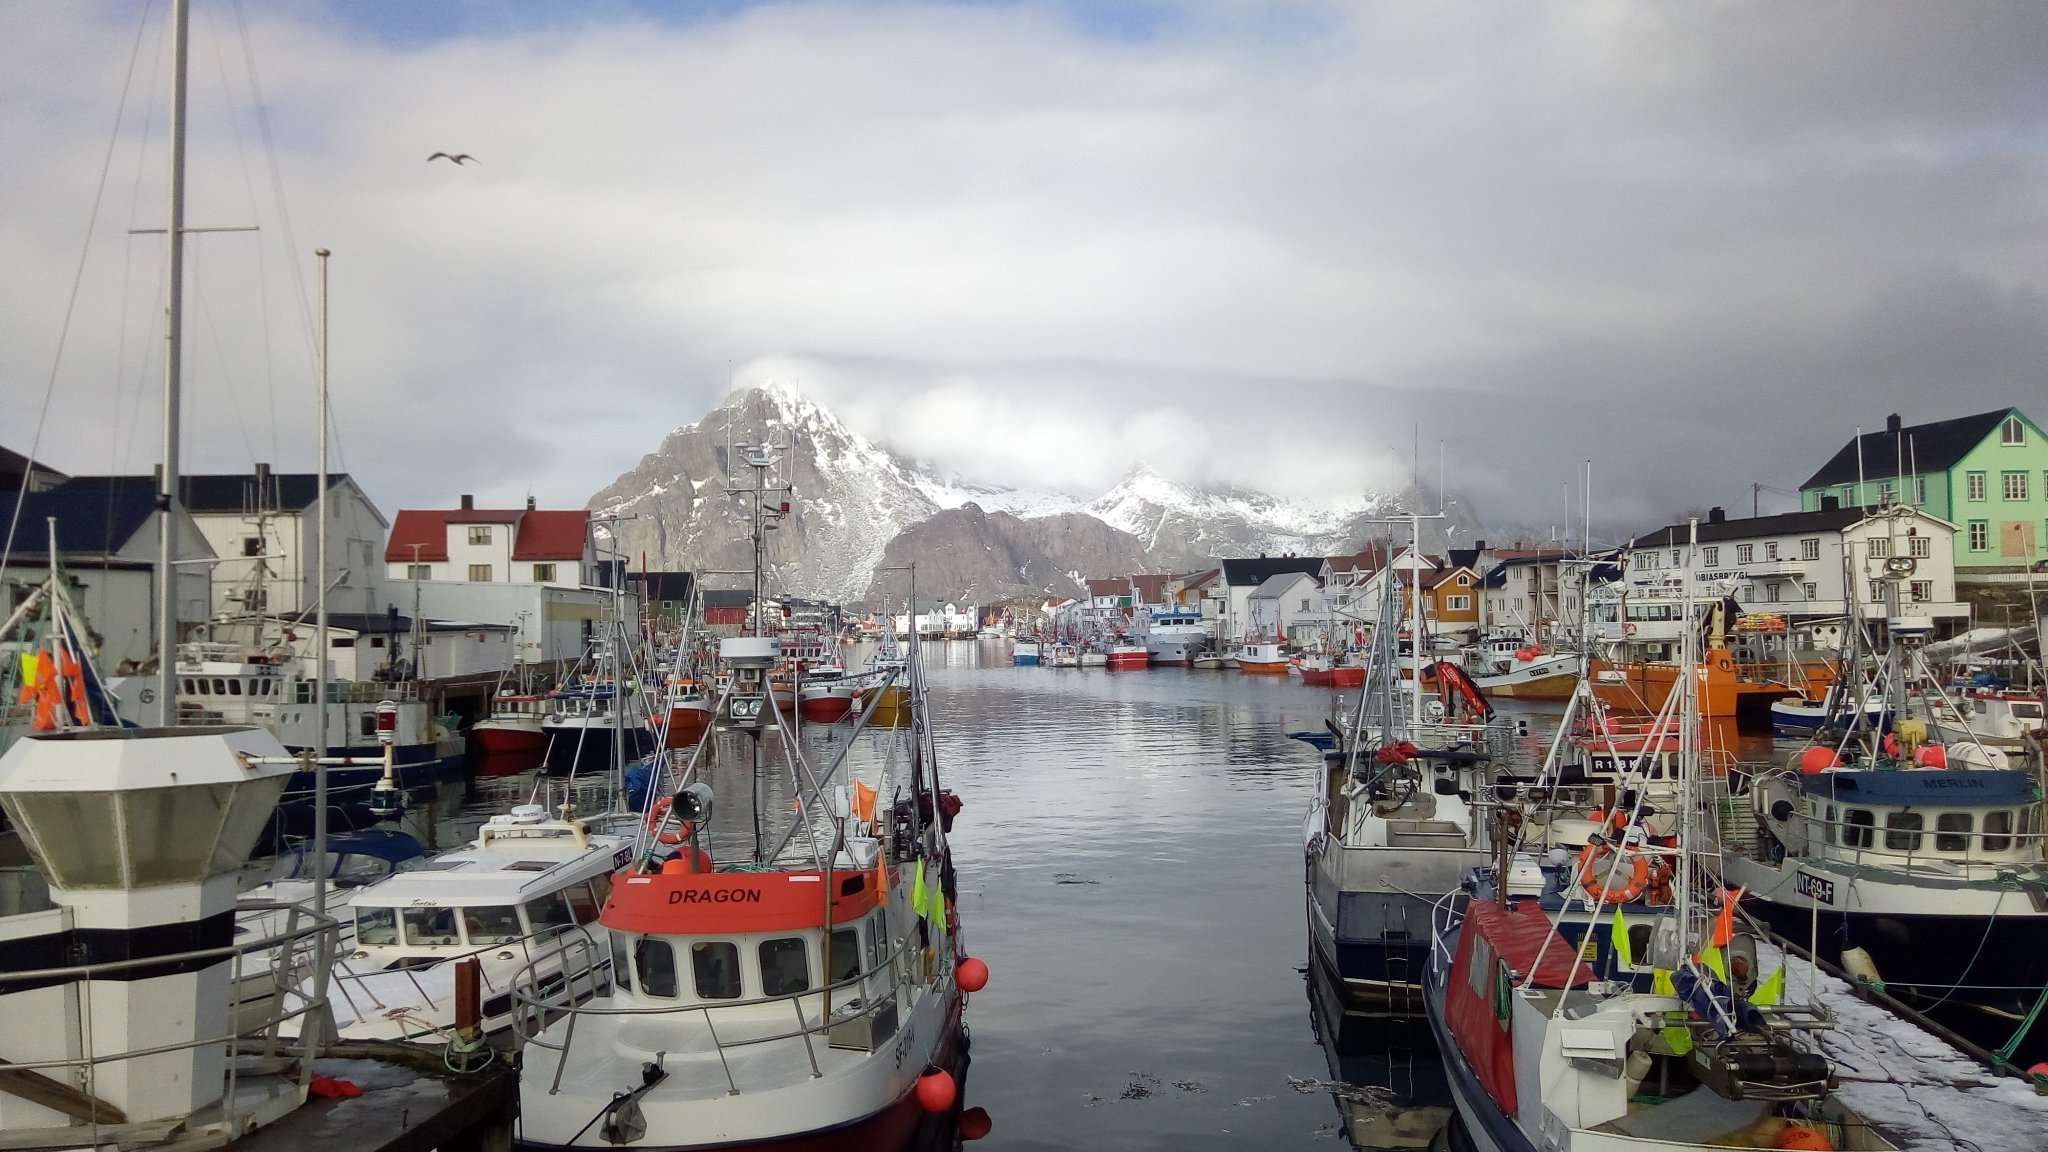
\includegraphics{/Users/marinaespinasse/github/ohi_norway_bookdown/pics/1553426042711.JPEG}

The growth in the blue economy is changing coastal ecosystems and communities in northern Norway. To guide ecosystem-based management, decision-makers need measures of ocean health and an analyzis of how industrial development affects sustainability of the human-ocean interactions.\\
{\textbf{The Ocean Health Index for Northern Norway (Coastal barometer)}} proposes a set of sustainability indicators that are measuring
the progress towards societal sustainability goals related to the coast, and evaluates the effect of coastal industries on these sustainability goals.

The study area of the project covers 81 coastal municipalities in northern Norway:

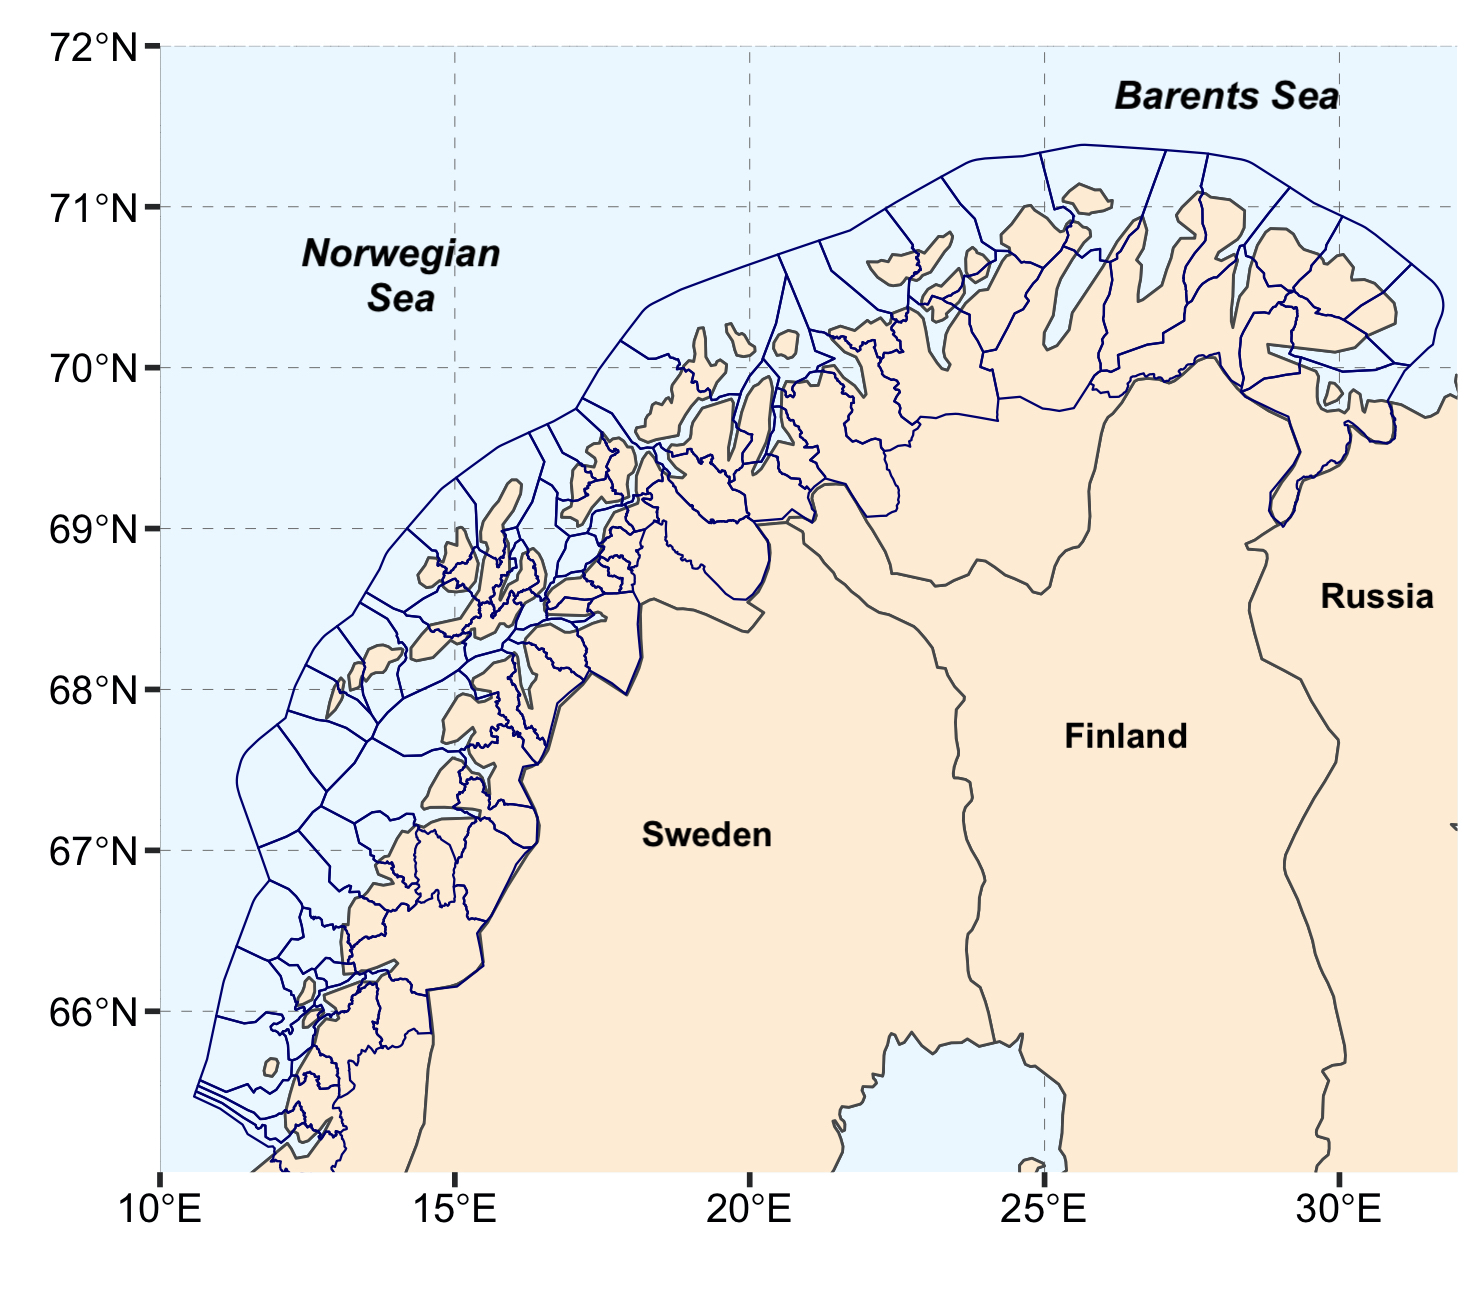
\includegraphics{/Users/marinaespinasse/github/ohi_norway_bookdown/pics/municipalities_map_labelled.jpg}

To learn more about the project, please visit our \href{https://markdownmonster.west-wind.com/docs/_4xs10gaui.htm}{blogg}.

\hypertarget{food}{%
\chapter{Food provision goal}\label{food}}

\hypertarget{aquaculture-sub-goal}{%
\section{Aquaculture sub-goal}\label{aquaculture-sub-goal}}

Aquaculture index measures sustainable production of farmed fish in northern Norway.
The table below explains the structure of aquaculture goal: the components of the goal and the data layers used to estimate them.

\begin{longtable}[]{@{}llll@{}}
\caption{\label{tab:simple-table} Data layers used for aquaculture sub-goal}\tabularnewline
\toprule
\begin{minipage}[b]{0.23\columnwidth}\raggedright
Component of the goal\strut
\end{minipage} & \begin{minipage}[b]{0.22\columnwidth}\raggedright
Data layers description\strut
\end{minipage} & \begin{minipage}[b]{0.25\columnwidth}\raggedright
Temporal coverage\strut
\end{minipage} & \begin{minipage}[b]{0.18\columnwidth}\raggedright
Data source\strut
\end{minipage}\tabularnewline
\midrule
\endfirsthead
\toprule
\begin{minipage}[b]{0.23\columnwidth}\raggedright
Component of the goal\strut
\end{minipage} & \begin{minipage}[b]{0.22\columnwidth}\raggedright
Data layers description\strut
\end{minipage} & \begin{minipage}[b]{0.25\columnwidth}\raggedright
Temporal coverage\strut
\end{minipage} & \begin{minipage}[b]{0.18\columnwidth}\raggedright
Data source\strut
\end{minipage}\tabularnewline
\midrule
\endhead
\begin{minipage}[t]{0.23\columnwidth}\raggedright
Production\strut
\end{minipage} & \begin{minipage}[t]{0.22\columnwidth}\raggedright
Standing biomass of salmon and trout per municipality each month; amount of fish lost during the production\strut
\end{minipage} & \begin{minipage}[t]{0.25\columnwidth}\raggedright
2005-2018\strut
\end{minipage} & \begin{minipage}[t]{0.18\columnwidth}\raggedright
The Fisheries Directorate of Norway\strut
\end{minipage}\tabularnewline
\begin{minipage}[t]{0.23\columnwidth}\raggedright
Fish lost during production\strut
\end{minipage} & \begin{minipage}[t]{0.22\columnwidth}\raggedright
Amount of fish died, escaped or lost due to other reasons during production each year\strut
\end{minipage} & \begin{minipage}[t]{0.25\columnwidth}\raggedright
2005-2018\strut
\end{minipage} & \begin{minipage}[t]{0.18\columnwidth}\raggedright
The Fisheries Directorate of Norway\strut
\end{minipage}\tabularnewline
\begin{minipage}[t]{0.23\columnwidth}\raggedright
Lice abundance\strut
\end{minipage} & \begin{minipage}[t]{0.22\columnwidth}\raggedright
Average lice abundance at a farm, compared to thresholds abundance\strut
\end{minipage} & \begin{minipage}[t]{0.25\columnwidth}\raggedright
2005-2018\strut
\end{minipage} & \begin{minipage}[t]{0.18\columnwidth}\raggedright
Norwegian Marine Data Center, Barentswatch.no portal\strut
\end{minipage}\tabularnewline
\begin{minipage}[t]{0.23\columnwidth}\raggedright
MOM B examinations\strut
\end{minipage} & \begin{minipage}[t]{0.22\columnwidth}\raggedright
The category of environmental impact at a farm from very good (1) to bery bad (4)\strut
\end{minipage} & \begin{minipage}[t]{0.25\columnwidth}\raggedright
2005-2018\strut
\end{minipage} & \begin{minipage}[t]{0.18\columnwidth}\raggedright
The Fisheries Directorate of Norway\strut
\end{minipage}\tabularnewline
\begin{minipage}[t]{0.23\columnwidth}\raggedright
Economic feed conversion ratio (eFCR)\strut
\end{minipage} & \begin{minipage}[t]{0.22\columnwidth}\raggedright
Consumption of feed per municipality each year\strut
\end{minipage} & \begin{minipage}[t]{0.25\columnwidth}\raggedright
2005-2015\strut
\end{minipage} & \begin{minipage}[t]{0.18\columnwidth}\raggedright
The Fisheries Directorate of Norway\strut
\end{minipage}\tabularnewline
\bottomrule
\end{longtable}

\hypertarget{estimating-sustainable-aquacultlure}{%
\subsection{Estimating sustainable aquacultlure}\label{estimating-sustainable-aquacultlure}}

Aquaculture goal consists of two components: total production and sustainability indices. When both components are calculated, they are combined into the amount of aquaculture production (in tonns og kg) produced sustainably.

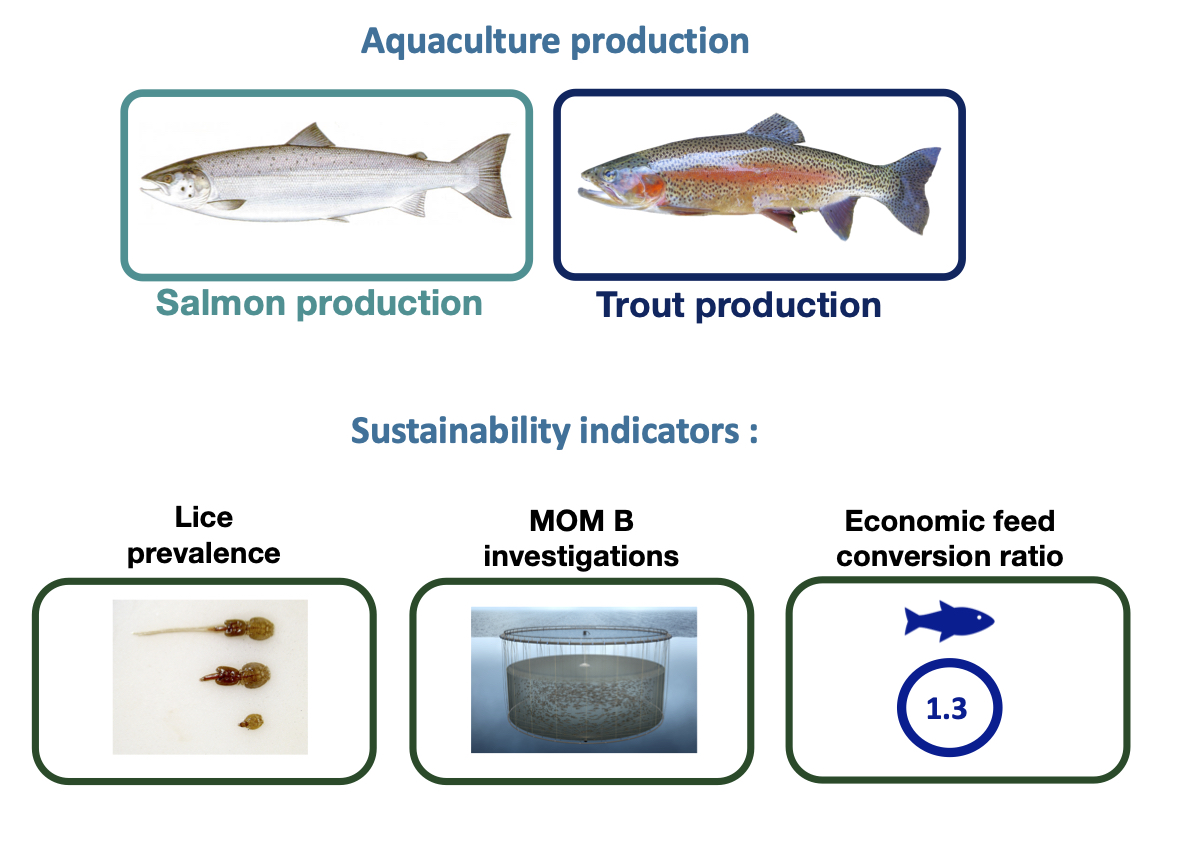
\includegraphics{/Users/marinaespinasse/github/ohi_norway_bookdown/pics/production_chart.jpg}

Below is the description of each component of the aquaculture sub-goal.

\textbf{Annual production}
We calculated total annual aquaculture production per municipality, as follows:
\(Tot.prod = \triangle Biomass + Harvest - Discard - Seeded\ smolts\)

Biomass change and harvest were corrected for slaughter weight, by multiplying their weight by 0.88.
The weight of smolts was assumed to be 100 grams, and the weight of discarded salmon - \textbf{5x0.88 = 4.4} kg.

Where, \(\triangle Biomass\) is the difference of standing biomass of fish in December of the given year minus December of the previous year, \(Harvest\) is biomass of fish harvested (kg); \(Seeded\ smolts\) is the biomass of smolts (kg), seeded for production at the beginning of the production cycle; \(Discard\) is the biomass of fish (kg) discarded at the slaughter plant, and Removed is the biomass of fish (kg) removed from the cages for slaughtering at another location or for other reasons

\(\triangle Biomass\) is the difference between standing biomass of fish in December of a given year minus standing biomass in December of the previous year. When it was not possible to subtract standing biomass of the previous year, for instance, when there was no fish in the cages at the end of the previous year, we calculated the difference between earliest and latest month of the give year, when there were fish in the cages.

For some municipalities, the total annual aquacultlure production was negative, due to underestimnation of fish biomass. In these cases, the total production was set to a missing value (NA). These missing values were replaced with a nearest observed produciton (either of the previous or of the following year).
Of the 81 coastal municipalities in Northern Norway, 10 did not have aquaculture in any of the studied years (1994 - 2018):

\begin{itemize}
\tightlist
\item
  Andoy
\item
  Berlavag
\item
  Hemnes
\item
  Malselv
\item
  Prosanger
\item
  Rost
\item
  Tana
\item
  Vado
\item
  Vaeroy
\item
  Vardo
\end{itemize}

For code on estimation of aquaculture produciton, please
\href{https://ohi-norway.github.io/nor-prep/prep/food_provision/Mariculture/total_aquaculture_production_and_efcr_newdata_jan2020.html}{see here}.

\textbf{Economic feed conversion ratio (eFCR)}
Economic feed conversion ratio (eFCR) is the ratio of the amount of feed used during the produciton of fish, to the final biomass of fish released to the market \citep{boyd2007indicators}.

\(eFCR = \frac{Feed \ used,\ kg}{Biomass\ produced,\ kg}\)

We calculated eFCR as a ratio of total feed used for production in a county (Norwegian ``fylke''), to the total biomass of fish produced annually in the county. The total feed consumption and total biomass produced per region were calculated as a sum of feed consumption and produced biomass of all municipalities within the county.

To calulate eFCR-based sustainability indicator, we compared eFCR between the northern Norwegian counites for each year. The municipalities, located in the county with the lowest eFCR got the highest score, and the other counties, and municipalities located in them, eFCR score was calculated as 1 minus percentage of difference between the given county's eFCR and the minimal observed eFCR that year.

\textbf{Lice prevalence}

High lice prevalence at the aquaculture production site can cause a decrease in production rate and can also cause a higher lice infection pressure on wild salmonids \citep{bjorn2001salmon, nilsen2017vurdering}.
In this study, we used a lice indicator developed by the Norwegian Food Authority (www.Mattilsynet.no), which compares the average abundance of lice reported weekly, with a threshold abundance of lice. In northern Norway, the threshold abundance of lice is set to be 0.5 lice per fish for all weeks, except weeks 21 to 26, when the thresholds is lowered to 0.2 (FOR-2012-12-05-1140).

Based on the lice monitoring by the Norwegian Food authority, we formulated indicator for our study in the following way. For the highest lice sustainability score over a year, each municipality should have lower than the threshold lice count throughout a year. In other words, the target of lice sustainability index is to keep lice under control at any time during the production cycle. For each produdction site, we estimated the proportion of weeks in a year when lice abundance is below a threshold and averaged this estimate for all locations within a single municipality. Thus, when all the aquaculture locations in a municipality in a given year were below lice threshold during all 53 weeks of a year, the municipality scored 1 for the lice indicator. Conversely, a small number of weeks when abundance of lice at production sites was below threshold resulted in a lower score.

\(Lice \ index = \sum_{i = 1}^{N \ of \ sites}[\frac{n \ weeks\ below_ \ threshold}{total\ weeks}]\)

Missing values in lice score data were replaced with an average of the score over the recent 5 years with data, when more than 7 years of data were available. If only 7 or fewer year with data were available, we used all given years to calculate the average score and replace missing values with this score.
For details on computation of the lice score, please follow this \href{https://ohi-norway.github.io/nor-prep/prep/food_provision/Mariculture/lice_count_at_localities.html}{link}.

\textbf{Environmentlal monitoring - MOM B scores}

In Norway, Modelling-Ongrowing fish farm Monitoring type B (MOM B) is the main management program for the monitoring of environmental impact from fish farms \citep{ervik1997regulating}.

The MOM B investigation involves analysis of sediments, taken directly below the farms and from the area up to 15 m beyond the farm. Three groups of sediment parameters are analyzed in MOM B: the presence and diversity of macro-infauna of the benthic sediments, pH and redox potential of the sediments, and sensory sediment variables (color, smell, consistency, gas ebullition, sludge thickness) (Norsk Standard 2016). This investigation is done less frequently than MOM A, usually one a year or every 2nd year but more frequently if high environmental impact was observed at the farm during the last monitoring \citep{norge2016miljoovervaaking}.

The producers are obliged to regularly run MOM B and report environmental status at their farms to the Fisheries Directorate of Norway. The outcome of the MOM B investigation is then scaled from 1 to 4, corresponding to very good, good, bad, and very bad environmental condition, respectively. When environmental impact at the farm is suspected to be bad (score 3 or 4), the Directorate can request an additional, and larger investigation of the environmental status (MOM C). When both investigations suggest a very bad environmental status at the farm, the Directorate may request to cease production until environmental conditions are improved (FOR-2008-06-17-822).

In this study, we used the scores of MOM B investigations to formulate the environmental impact index of aquaculture sustainability. We assumed that the extent of environmental impact from the production on the surrounding environment increases with the size of the farm, which is reflected in the maximal allowed production biomass (MAB). To estimate the environmental impact index, we calculated the sum of biomass of all the locations that scored 3 and 4 at the MOM B investigations, per municipality and year. Then, we calculated the proportion of this biomass to total biomass of all the farms located in a municipality each year, and 1 minus this proportion returned an environmental impact sustainability index.

\(MOMB \ index = 1 - (\frac{MTB_{frams \ scored \ 3 \ and \ 3}}{MTB_{municipality \ total}})\)

The resultant index can be interpreted as follows. For a highest score, all the production sites within a municipality should score 1 or 2 at MOM B investigations. Also, the lower the biomass and number of the sites that score 3 and 3 at MOM B, the higher the score.

\hypertarget{carbon-storage}{%
\chapter{Carbon storage}\label{carbon-storage}}

Here is a review of existing methods.

\hypertarget{clean-waters}{%
\chapter{Clean waters}\label{clean-waters}}

We describe our methods in this chapter.

  \bibliography{book.bib,packages.bib}

\end{document}
